\documentclass{standalone}
\usepackage[utf8]{inputenc}
\usepackage[T1]{fontenc}
\usepackage[turkish]{babel}
\usepackage{tikz}
\usetikzlibrary{arrows.meta,shapes}
\begin{document}
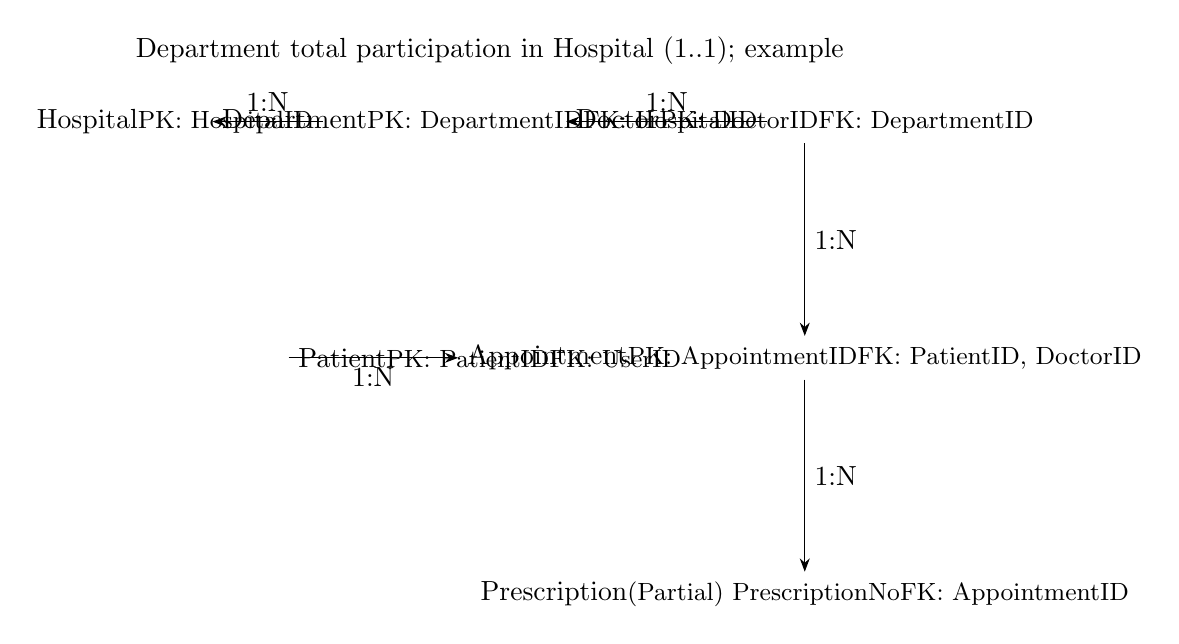
\begin{tikzpicture}
  % styles
  \tikzset{
    entity/.style={draw, rectangle, minimum width=3.2cm, minimum height=0.9cm, align=center},
    weak/.style={draw, rectangle, double, minimum width=3.2cm, minimum height=0.9cm, align=center}
  }

  % nodes
  \node[entity] (Hospital) at (0,0) {Hospital\\{\small PK: HospitalID}};
  \node[entity] (Department) at (4,0) {Department\\{\small PK: DepartmentID\\FK: HospitalID}};
  \node[entity] (Doctor) at (8,0) {Doctor\\{\small PK: DoctorID\\FK: DepartmentID}};
  \node[entity] (Patient) at (4,-3) {Patient\\{\small PK: PatientID\\FK: UserID}};
  \node[entity] (Appointment) at (8,-3) {Appointment\\{\small PK: AppointmentID\\FK: PatientID, DoctorID}};
  \node[weak] (Prescription) at (8,-6) {Prescription\\{\small (Partial) PrescriptionNo\\FK: AppointmentID}};

  % relations / cardinalities
  \draw[-{Stealth}] (Hospital) -- node[above]{1:N} (Department);
  \draw[-{Stealth}] (Department) -- node[above]{1:N} (Doctor);
  \draw[-{Stealth}] (Patient) -- node[below]{1:N} (Appointment);
  \draw[-{Stealth}] (Doctor) -- node[right]{1:N} (Appointment);
  \draw[-{Stealth}] (Appointment) -- node[right]{1:N} (Prescription);

  % participation note
  \node at (4,0.9) {Department total participation in Hospital (1..1); example};
\end{tikzpicture}
\end{document}
